
The world faces significant challenges from climate change and global warming \cite{Masson-Delmotte2018}. A rise in carbon emissions increases the risk of severe impacts on the world such as rising sea levels, species extinction, heat waves and tropical cyclones \cite{IPCC2014}. The scientific literature concurs that the recent change in climate is anthropogenic, with 97\% of peer reviewed articles of this view \cite{Cook2013}.  

As shown by Figure \ref{fig:fuel_emissions_market_share}, the electricity mix is dominated by high carbon emitting fuels such as coal and natural gas. Low-carbon solutions, such as nuclear, renewables and hydro, combine to produce less electricity than solely coal as a fuel source. 



\begin{figure}[b]
	\begin{center}
		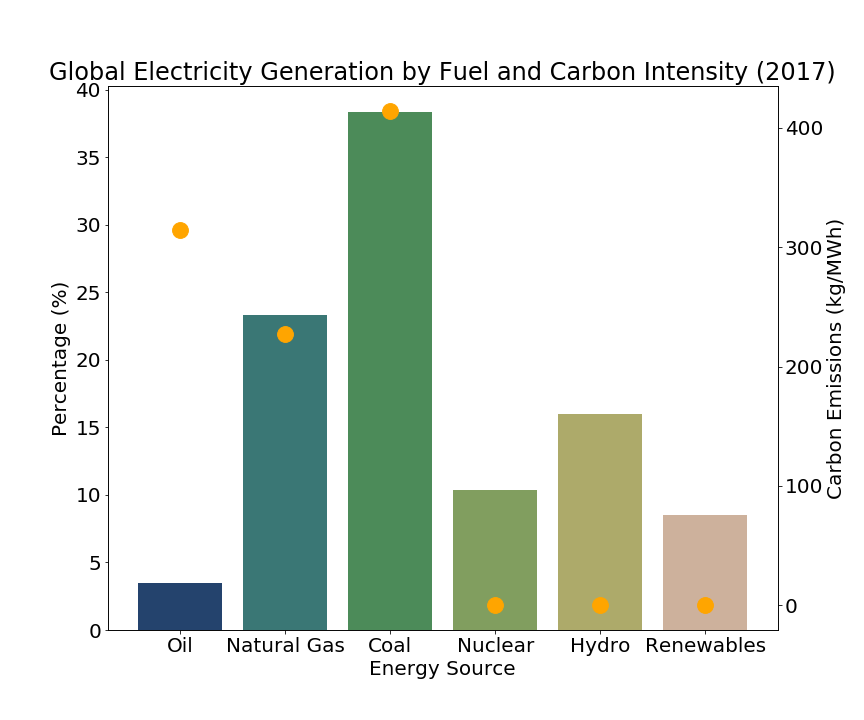
\includegraphics[width=0.45\textwidth]{figures/elec_gen_carbon.png}
		\caption{Global electricity generation sources and relative carbon emission intensity. ~\cite{BP2018,Hall1983}}
		\label{fig:fuel_emissions_market_share}
	\end{center}
\end{figure}


To achieve a low carbon energy infrastructure, and limit the effects of global warming, a transition in the electricity mix is required. Moving from a centralised and homogenous fossil fuel-based system to a distributed system based on renewable energy and batteries. Batteries are required due to the fact that most renewable sources are effected by conditions outside the control of the owners (e.g. time of day, wind speed and cloud cover). This leads to a need for electricity to be stored at times of low electricity demand and high renewable resources, and for the batteries to be discharged at times of high demand and low supply. 

Such a transition needs to be performed in a safe and non-disruptive manner -- it may be possible to close down all fossil fuel plants in the next year, though if this leads to electricity shortages and power cuts then this is likely to cause significant problems both for companies and homes. Therefore a stepped approach which allows seamless transfer is desirable. This may seem a simple process to achieve -- slowly phase out existing fossil fuel generators and replace these by renewable sources -- however, there are many risks and uncertainties in this process. Existing power plants have an expected lifetime and their owners wish to maximise this and the profits which can be made from them, renewable sources are still developing -- meaning that their efficiency and reliability will change in years to come.

Due to the long construction times, long operating periods and high costs of power plants, investment decisions made today can have long term impacts on future electricity supply \cite{Chappin2017}. Governments, and society, therefore have a role in ensuring that the negative externalities of pollution and carbon emission are priced into electricity generation so that optimal decisions are made. Due to the absence of central control in electricity generation investment, other methods must be used to influence the independent players of the electricity market. Methods such as carbon taxes, policy and regulation can aid in the goals of reducing carbon emissions to limit global warming, as agreed in the Paris agreement \cite{May2002}.

A common method to understand and reduce risk and uncertainty, especially in electricity planning, is simulation and modelling. Simulation and modelling allows practitioners to realise a physical system in a virtual model. In this context, a model is defined as an approximation of a system through the use of mathematical formulas and algorithms. Through simulation it is possible to test a system where real life experimentation would not be practical due to reasons such as prohibitively high costs, time constraints or risk of detrimental impacts. This has the dual benefit of minimising the risk of real decisions in the physical system, as well as allowing practitioners to test less risk-averse strategies. Without simulation one would frequently make safer decisions to reduce risk.

Agent-based modelling (ABM) is a class of computational simulation models composed of autonomous, interacting agents. ABMs are a way of modelling the dynamics of a complex system \cite{MacAl2010}. Due to the numerous and diverse actors involved in the generation, distribution and sale of electricity in liberalised electricity markets, agent based models are well suited and increasingly being used in the literature \cite{Zhou2007}.


In this paper, we present ElecSIM, an open-source agent-based model that simulates generation companies (GenCos) in an electricity market. ElecSIM models GenCos as multiple agents and electricity demand as a single aggregated agent, with a power exchange that facilitates trades between the two. 

GenCos actively make bids for each of the power plants they own to match demand. Their bids are based on their costs to supply a single unit (1MWh) of electricity, known as their short run marginal cost (SRMC), which excludes capital and fixed costs. The power exchange links bids to supply based on merit-order, with priority to the cheapest bids first. GenCos then invest in power plants based on expected profitability of each option.


Through simulation we can evaluate many strategies in order to identify those most likely to achieve our goals of rapid but non-disruptive migration from fossil to renewable.






ElecSIM can be used by:
\begin{itemize}
	\item {\bf Policy experts} to test policy outcomes under different scenarios and provide quantitative advice to policy makers. They can provide a simple script defining the policies they wish to use along with the parameters for these polices.
	\item {\bf Energy market developers} who can use the extensible framework to add such things as new energy sources, policy types, consumer profiles and storage types. Thus allowing ElecSIM to adapt to a changing ecosystem.
\end{itemize}




 {\color{red} A diagram showing the different players, who can influence them and how?}

This paper details our model, ElecSIM. Section \ref{Literature Review} is a literature review of the models currently used in practice. Section \ref{Model} details the model and assumptions made, and section \ref{Valdiation and Performance} details how we validated our model, and displays performance metrics. Section \ref{Scenario Testing} details our results, and explores ways in which ElecSIM can be used. We conclude the work and propose future work in section \ref{Conclusion}.




%
%To achieve carbon neutrality, this electricity mix must shift from a largely fossil fuel based system, to one based on renewable energy. We must use solar, wind and tidal power to generate electricity to power homes, industry and transport \cite{Hoffert2002}. Electricity is a significant proportion of our energy consumption -- consuming 22\% of energy usage per year -- which must grow to meet the demands of a low-carbon transport and heating system \cite{Lakshmi2017}.  Although other forms of energy consumption are important we focus here only on the production and consumption of electricity. 


%\begin{itemize}
%	\item We have developed a framework for evaluating alternative scenarios, prior to implementation of policy.
%	\item Used by experts working in collaboration with policy makers.
%	\item Importance of a transition in electricity infrastructure (Paris agreement, UK Climate change act)
%	\item Importance of understanding effect of decisions made today on the future (limit of 1.5C by 2050)
%	\item Introduce ElecSIM as a toolkit to inform long-term domestic policy questions in the electricity market. 
%	\item Ability to model the effects of carbon taxation, and the effect of different scenarios 
%	\item Talk about the need to model a non-stationary, dynamic system, with multiple interacting agents with imperfect information
%	\item Requirement for an Open-Source, free Toolkit written in python. Low barrier of entry, and integration with existing python data analytics and machine learning techniques. Transparent, reproducible, and data made available. This allows for results to be open to greater criticism and better inform policy decisions.
%	\item Simple model which matches real life behaviour for low complexity and therefore increases transparency.
%\end{itemize}

